\documentclass[a4paper, fleqn]{article}

\usepackage{amsmath}
\usepackage{enumitem}
\usepackage{graphicx}

\begin{document}

\title{Lab Exercise III \\ Making Maps I: Introduction to Spatial Analysis, Data Visualization and Map Design}
\author{Basil R. Yap}
\date{2018 February 08}
\maketitle

\section{Part I}

\begin{itemize}
\item \textbf{Figure 1}: \begin{itemize}
\item Number of bikes in Singapore: 39215
\item Number of bikes in SUTD: 204
\end{itemize}
\begin{figure}[h!]
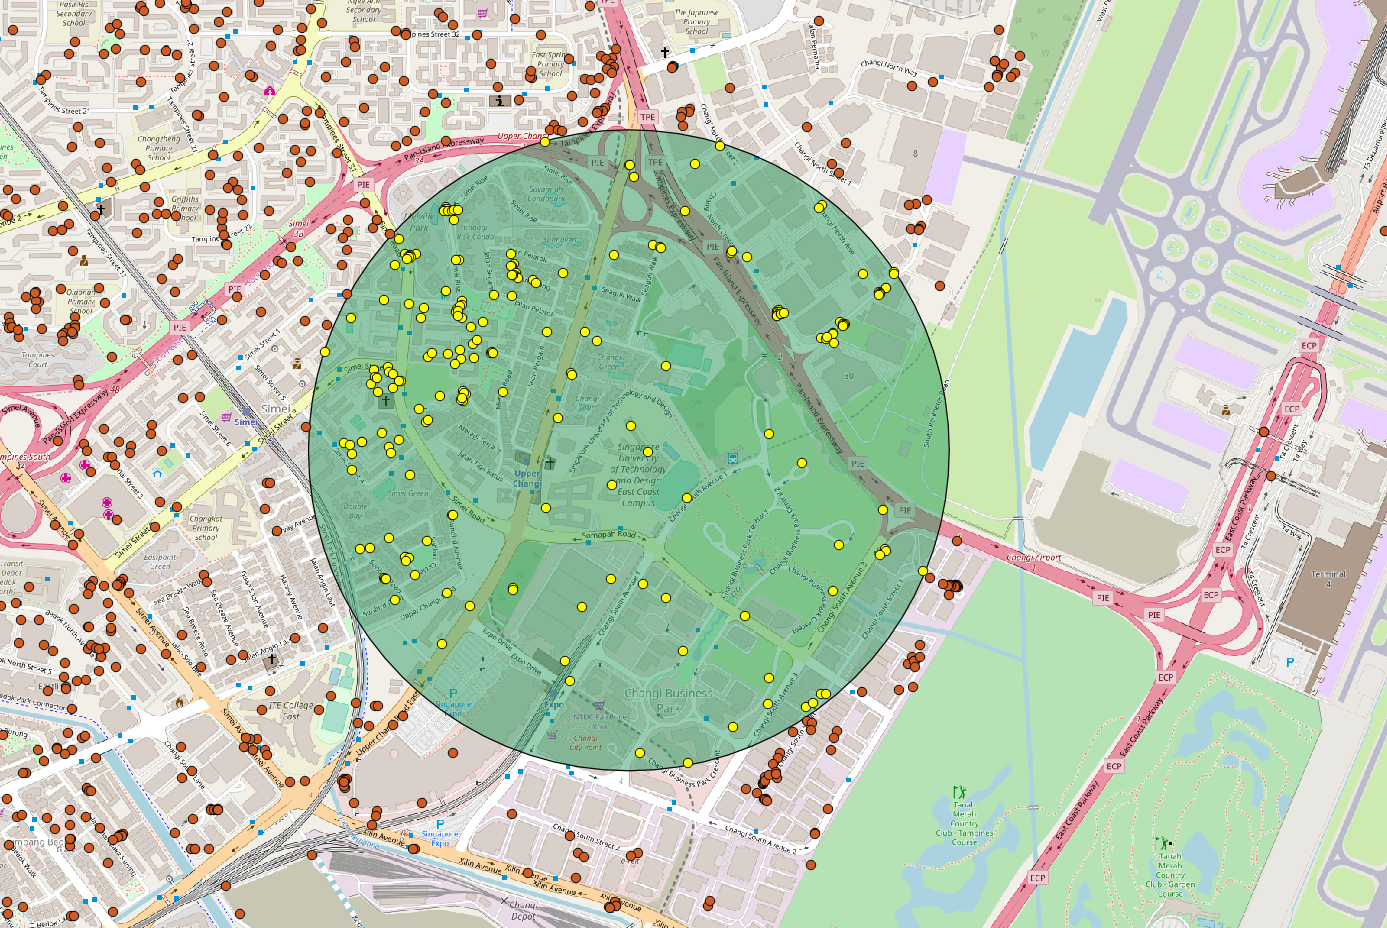
\includegraphics[width=\linewidth]{./assets/201802081725.png}
\caption{Bikes in Changi Business Park Area}
\label{figure:map1}
\end{figure}
\pagebreak
\item \textbf{Figure 2}: \begin{itemize}
\item Redhill
\item Boon Keng
\item Macpherson
\item Clementi
\item Jurong West
\item Chua Chu Kang
\end{itemize}
\begin{figure}[h!]
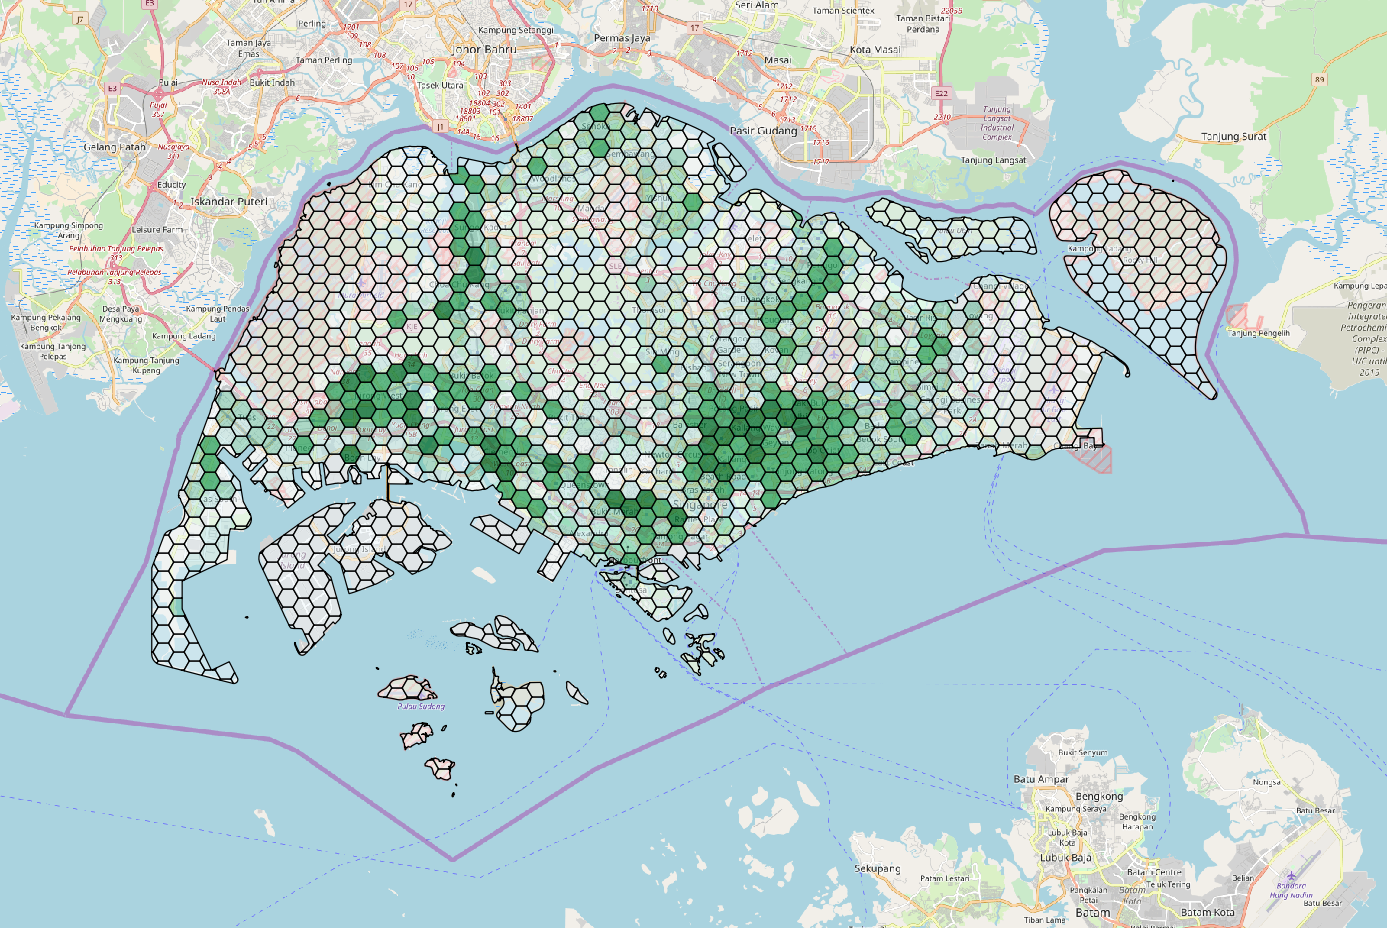
\includegraphics[width=\linewidth]{./assets/201802081800.png}
\caption{Bike Distribution in Singapore}
\label{figure:map2}
\end{figure}
\item \begin{itemize}
\item Mean: 28.5123726346
\item Median: 3.0
\item Max: 210.0
\end{itemize}
\pagebreak
\item \textbf{Figure 3}: Neighborhood around Tah Ching Road\\
\begin{figure}[h!]
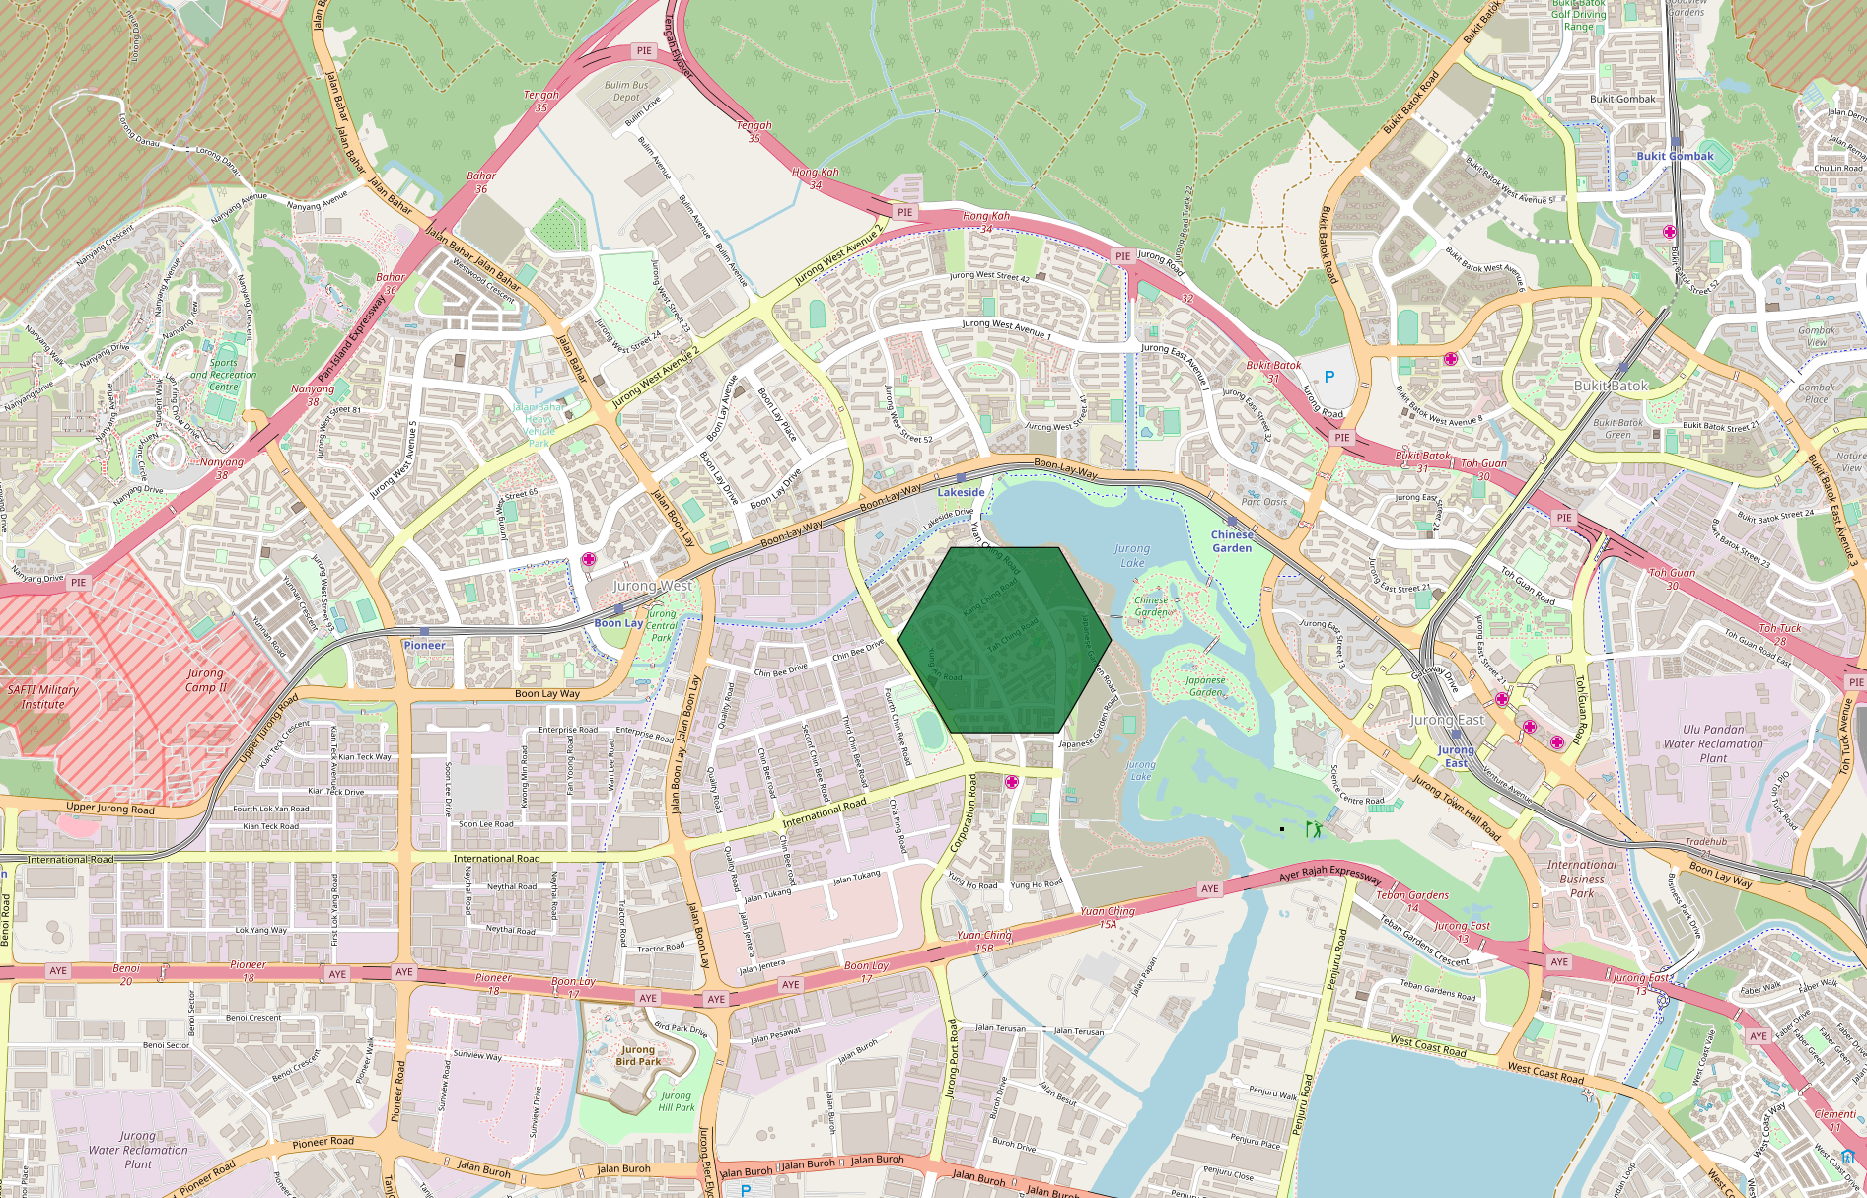
\includegraphics[width=\linewidth]{./assets/201802091815.png}
\caption{Tah Ching Road with 210 bikes around it}
\label{figure:map3}
\end{figure}
\pagebreak
\item \textbf{Figure 4}:\\
\begin{figure}[h!]
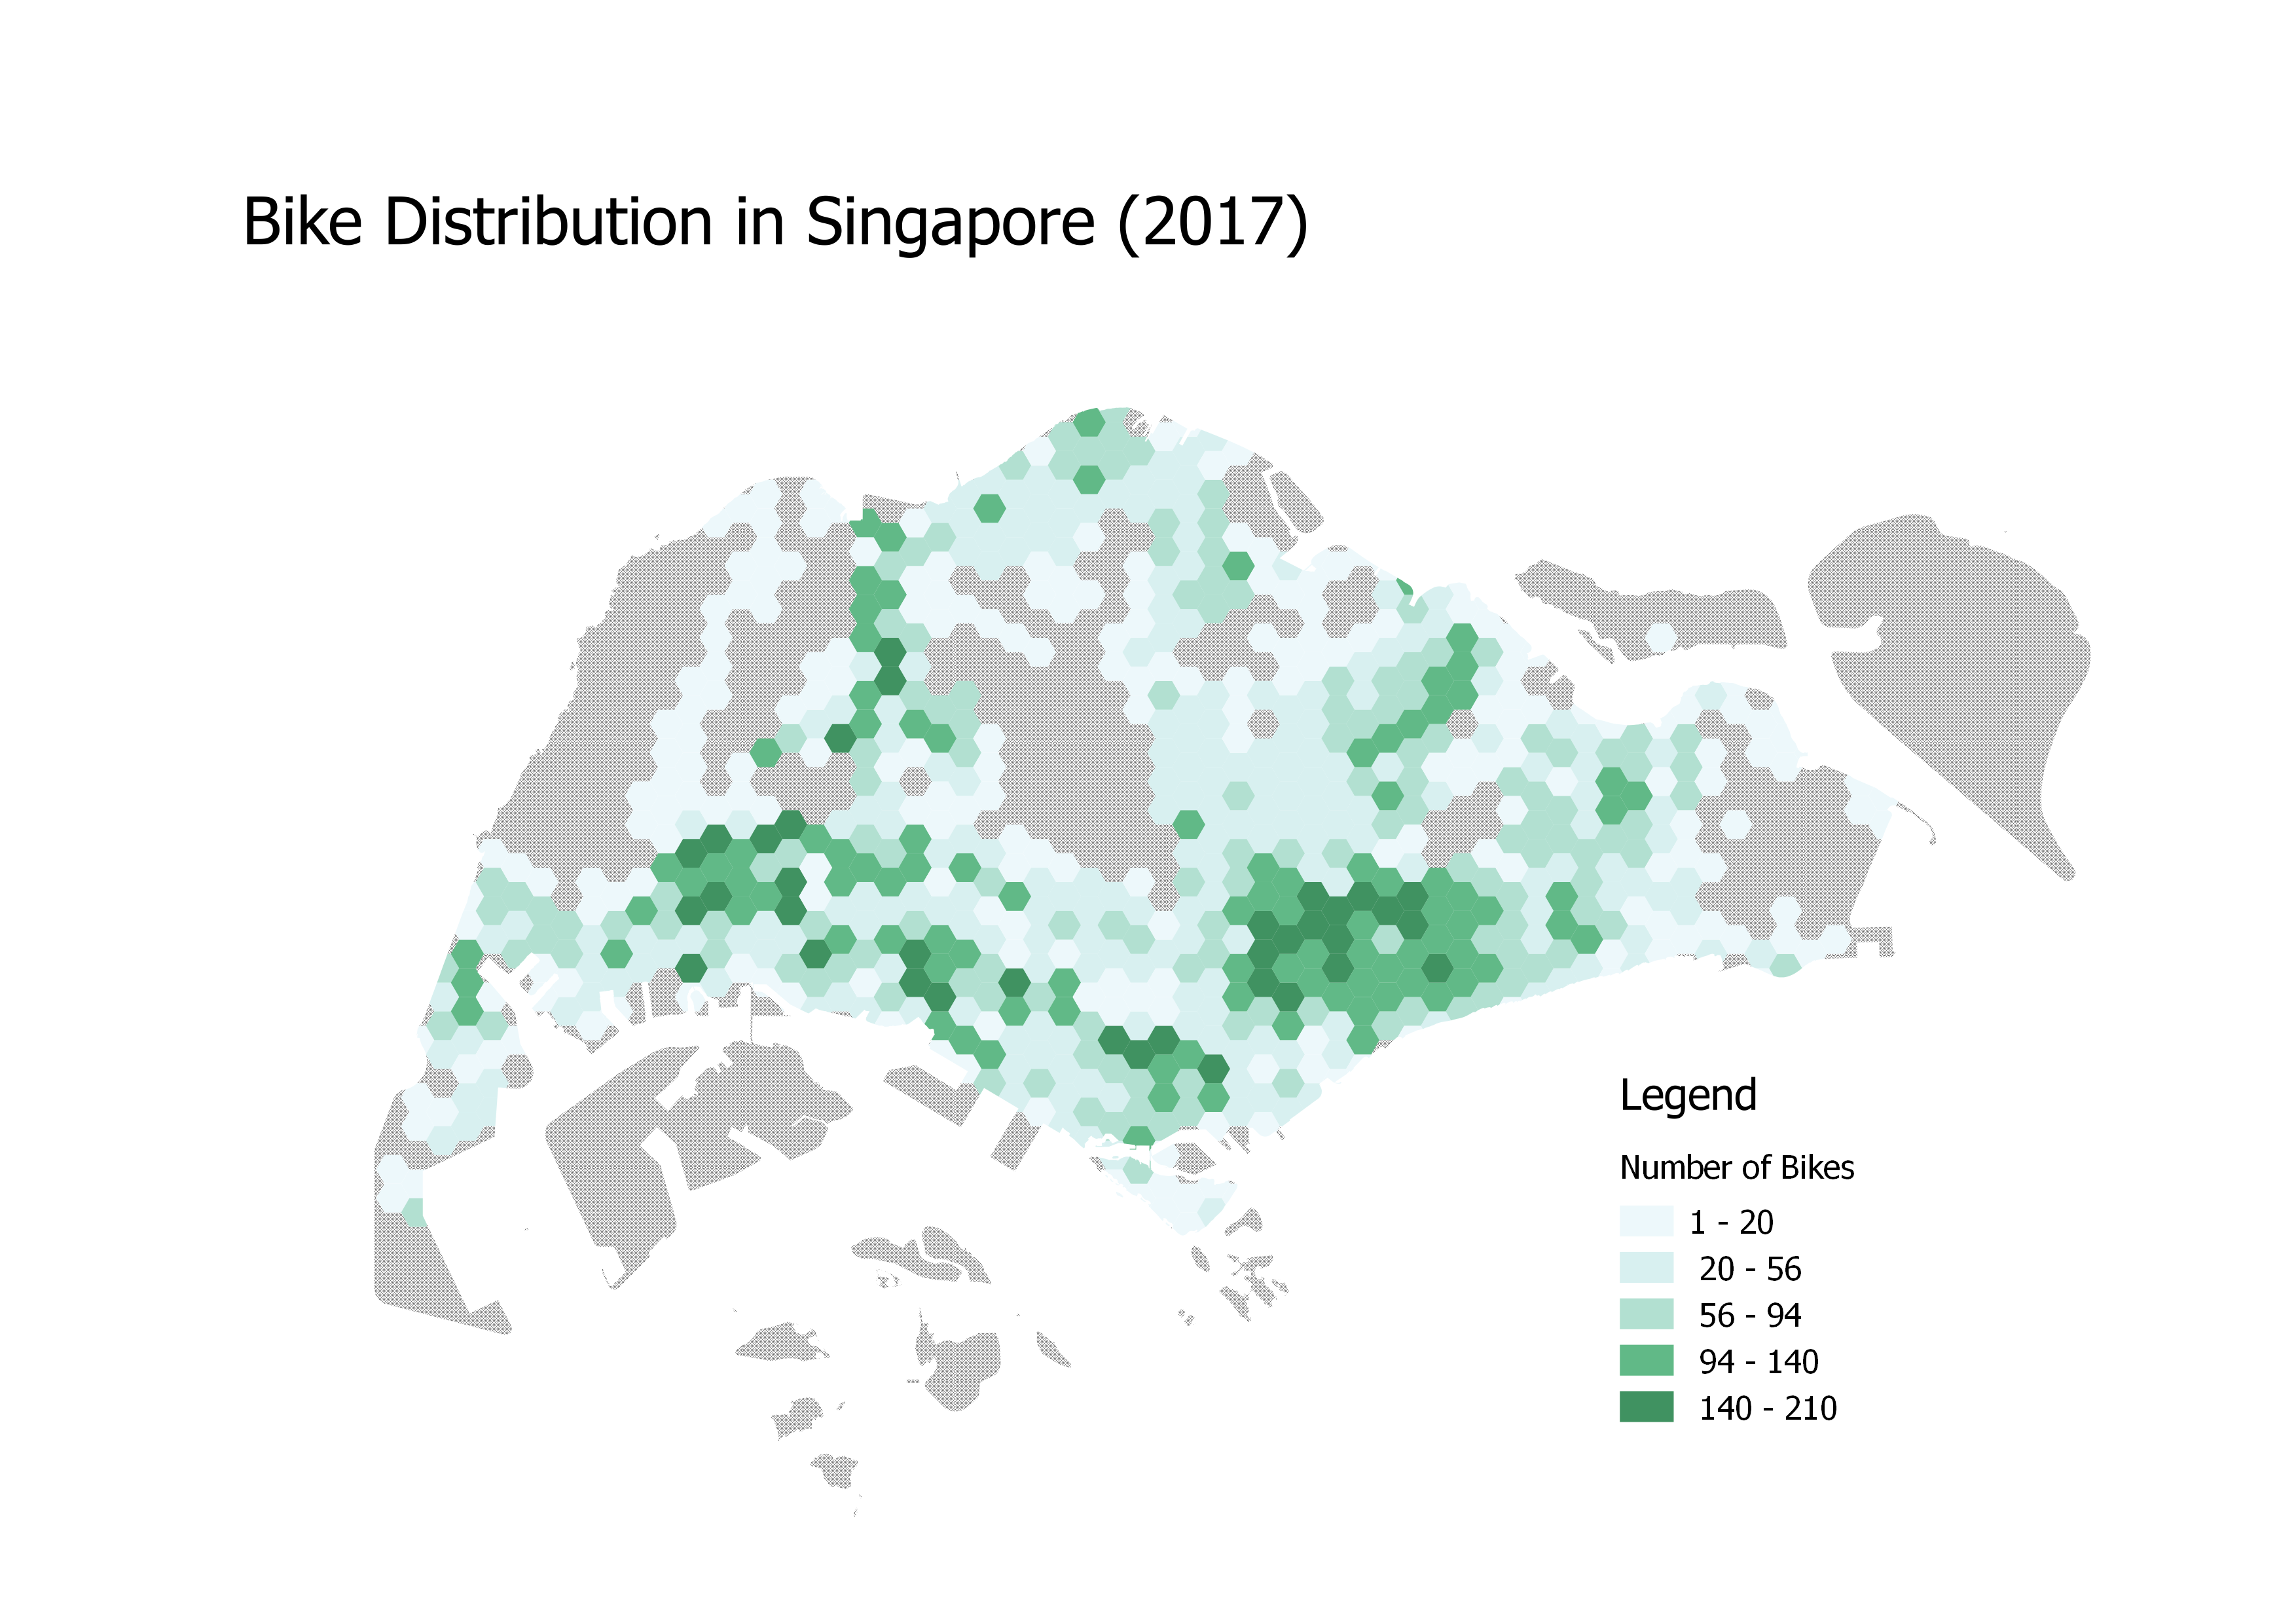
\includegraphics[width=\linewidth]{./assets/201802091838.png}
\caption{Bike Distribution in Singapore (2017)}
\label{figure:map4}
\end{figure}
\pagebreak
\item \textbf{Figure 5}:\\
From the two maps, we can two distinct differences:\begin{enumerate}
\item There are considerably less tiles with low concentrations of bike in Figure 5 than in Figure 4
\item There are some tiles that have higher concentration of bikes in Figure 5 than in Figure 4
\end{enumerate}
The lower concentrations support the initial hypothesis, which stated bikes tend to be parked near bus stops. Tiles that were further from the bus stops tend to have lower number of bikes.\\
Some tiles having increased concentrations may be due to varying concentrations of bus stops. Despite having an overall lower number of bikes per tile in Figure 4, the concentration of the bikes near bus stops show to be high in Figure 5. This means the ratio of bikes to bus stops in most tiles are high, further supporting our initial hypothesis.
\begin{figure}[h!]
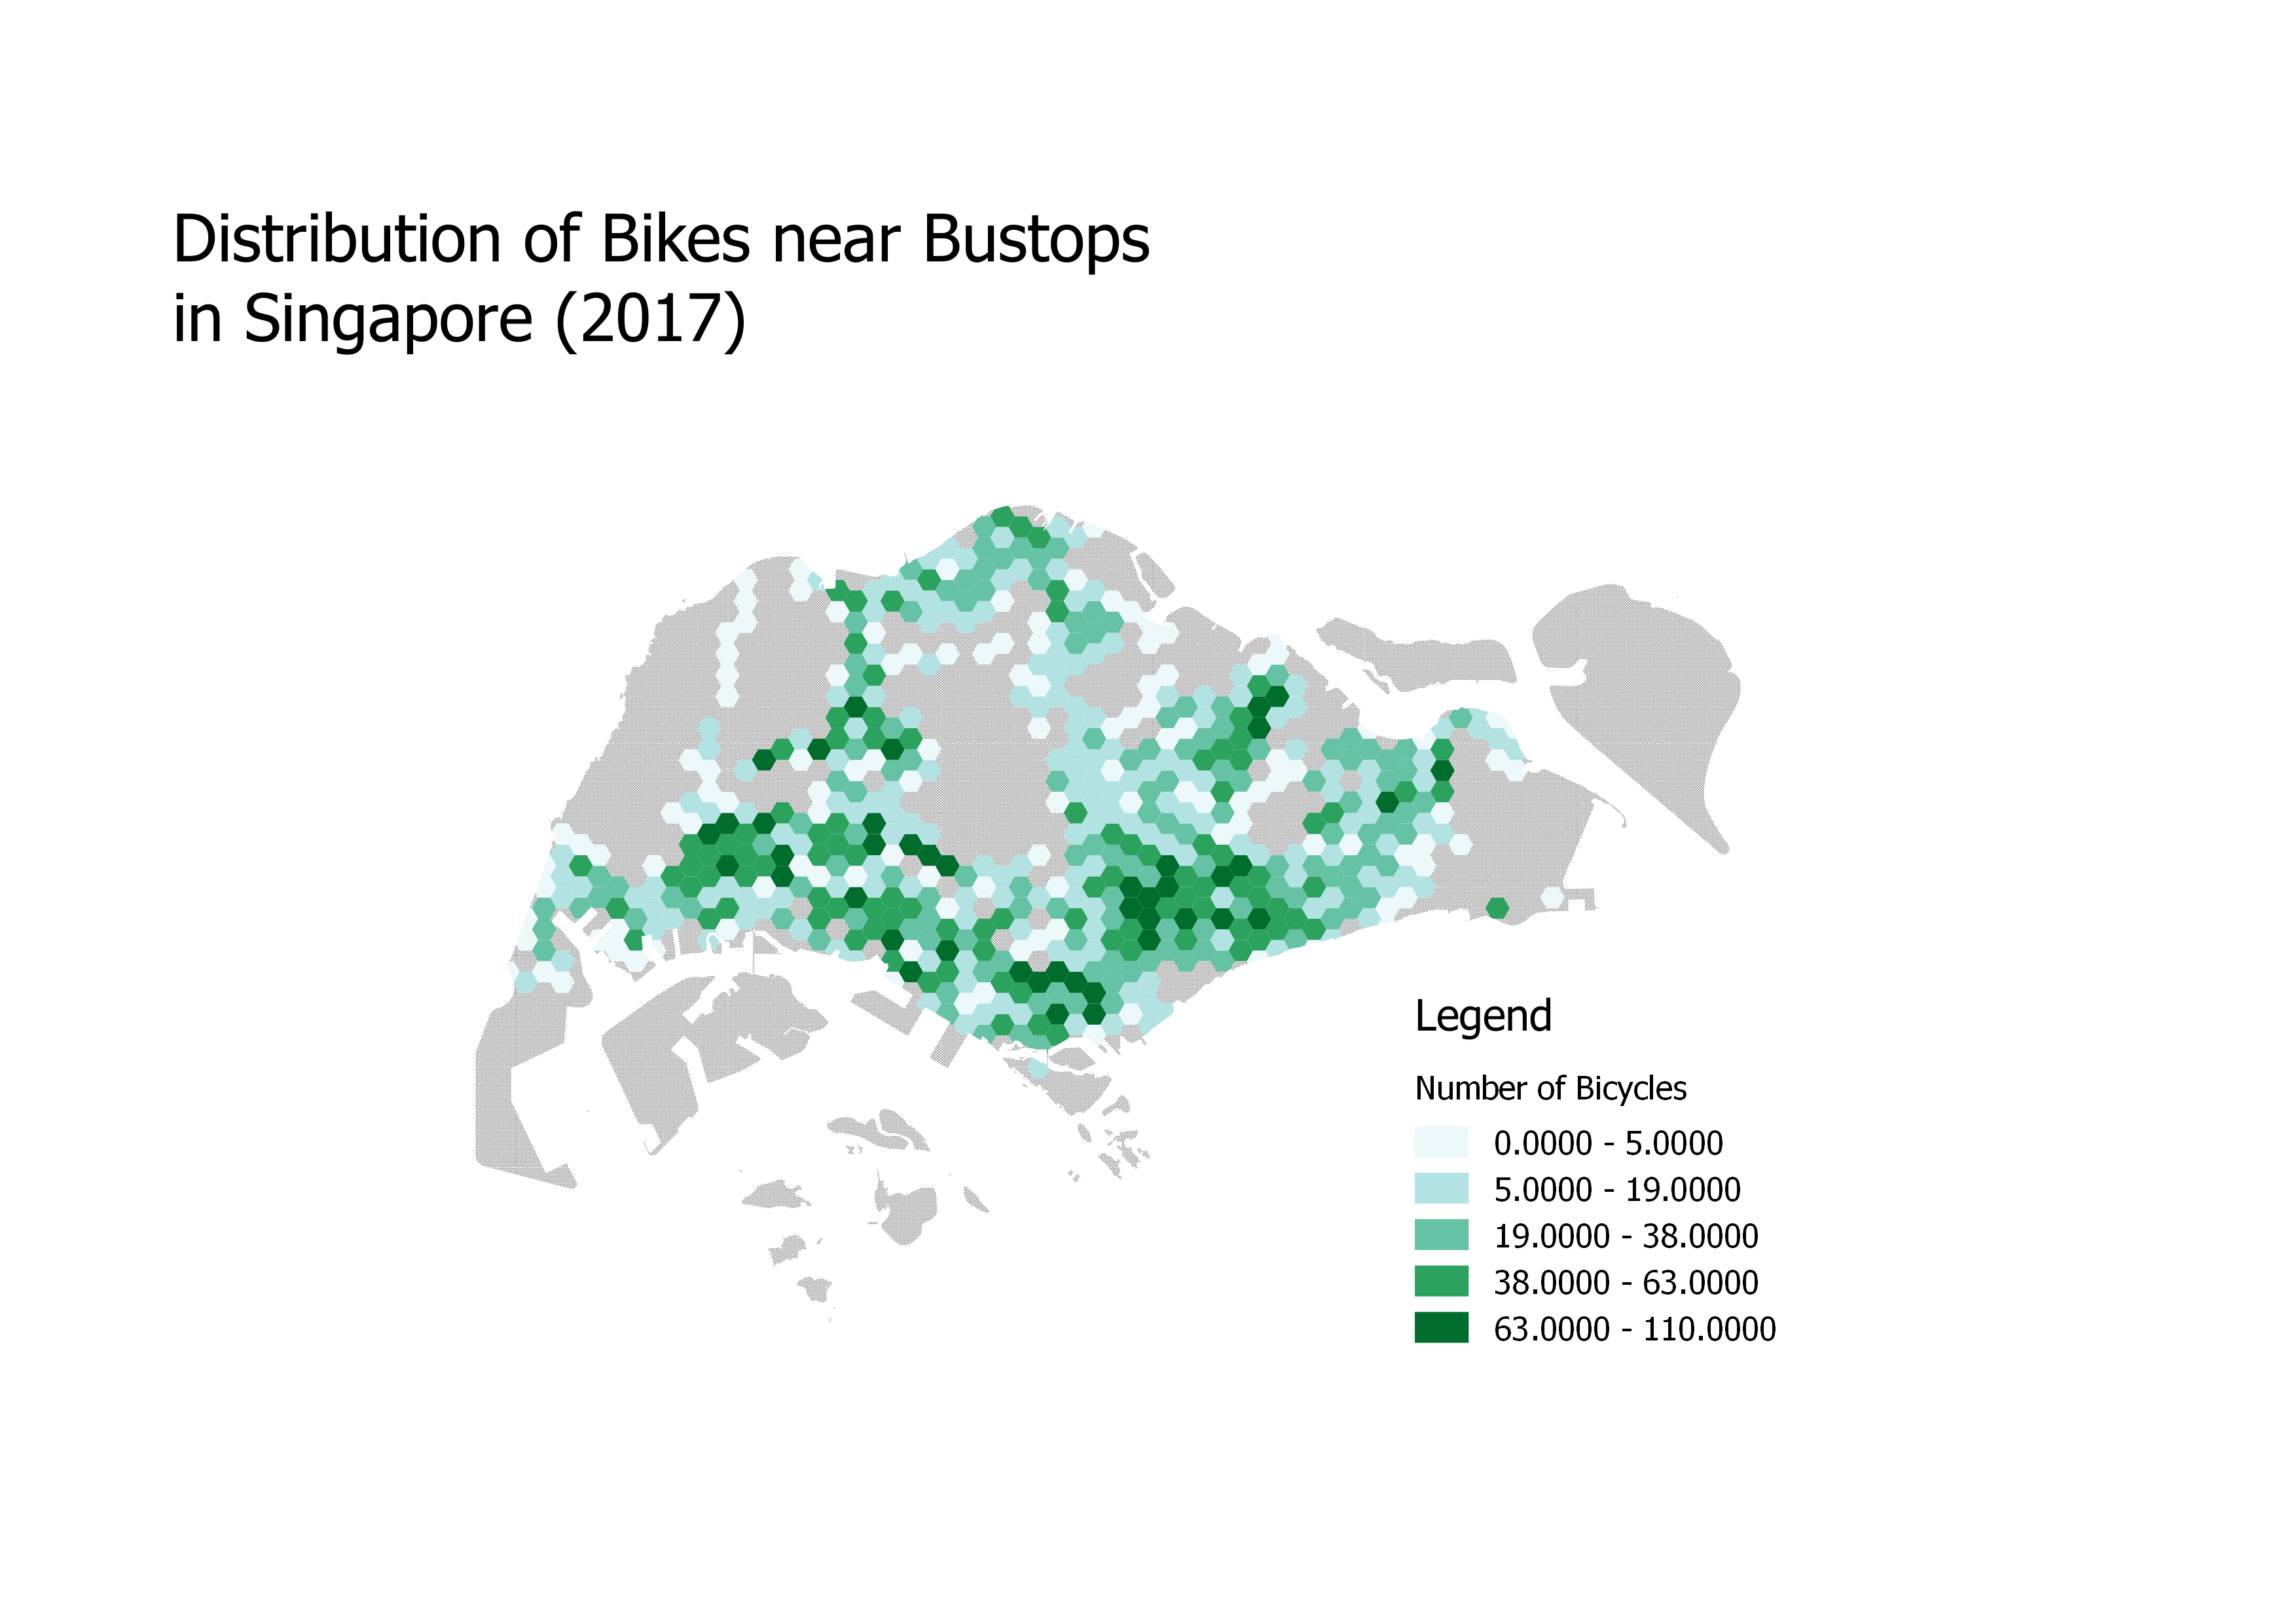
\includegraphics[width=\linewidth]{./assets/201802092119.png}
\caption{Distribution of Bikes near Busstops in Singapore (2017)}
\label{figure:map5}
\end{figure}
\pagebreak
\item \textbf{Figure 6 \& 7}: \\
From the maps, there is a clear abnormality in the data provided. Most of the missing bikes reported in Singapore are contained within the vicinity of a few HDB blocks. Despite the low number of reports, the abnormality is shown to be very substantial.\\
I would still choose not to publish this map, as the map itself is very incriminating to the residents of the few HDB blocks contained within it. Publishing the map would do more harm than good for all parties involved. By anonymizing the information or aggregating the points to a neighborhood level, the information would be sufficient for authorities to investigate the high number of missing bikes without jeopardizing the welfare of innocent parties.\\
\begin{figure}[h!]
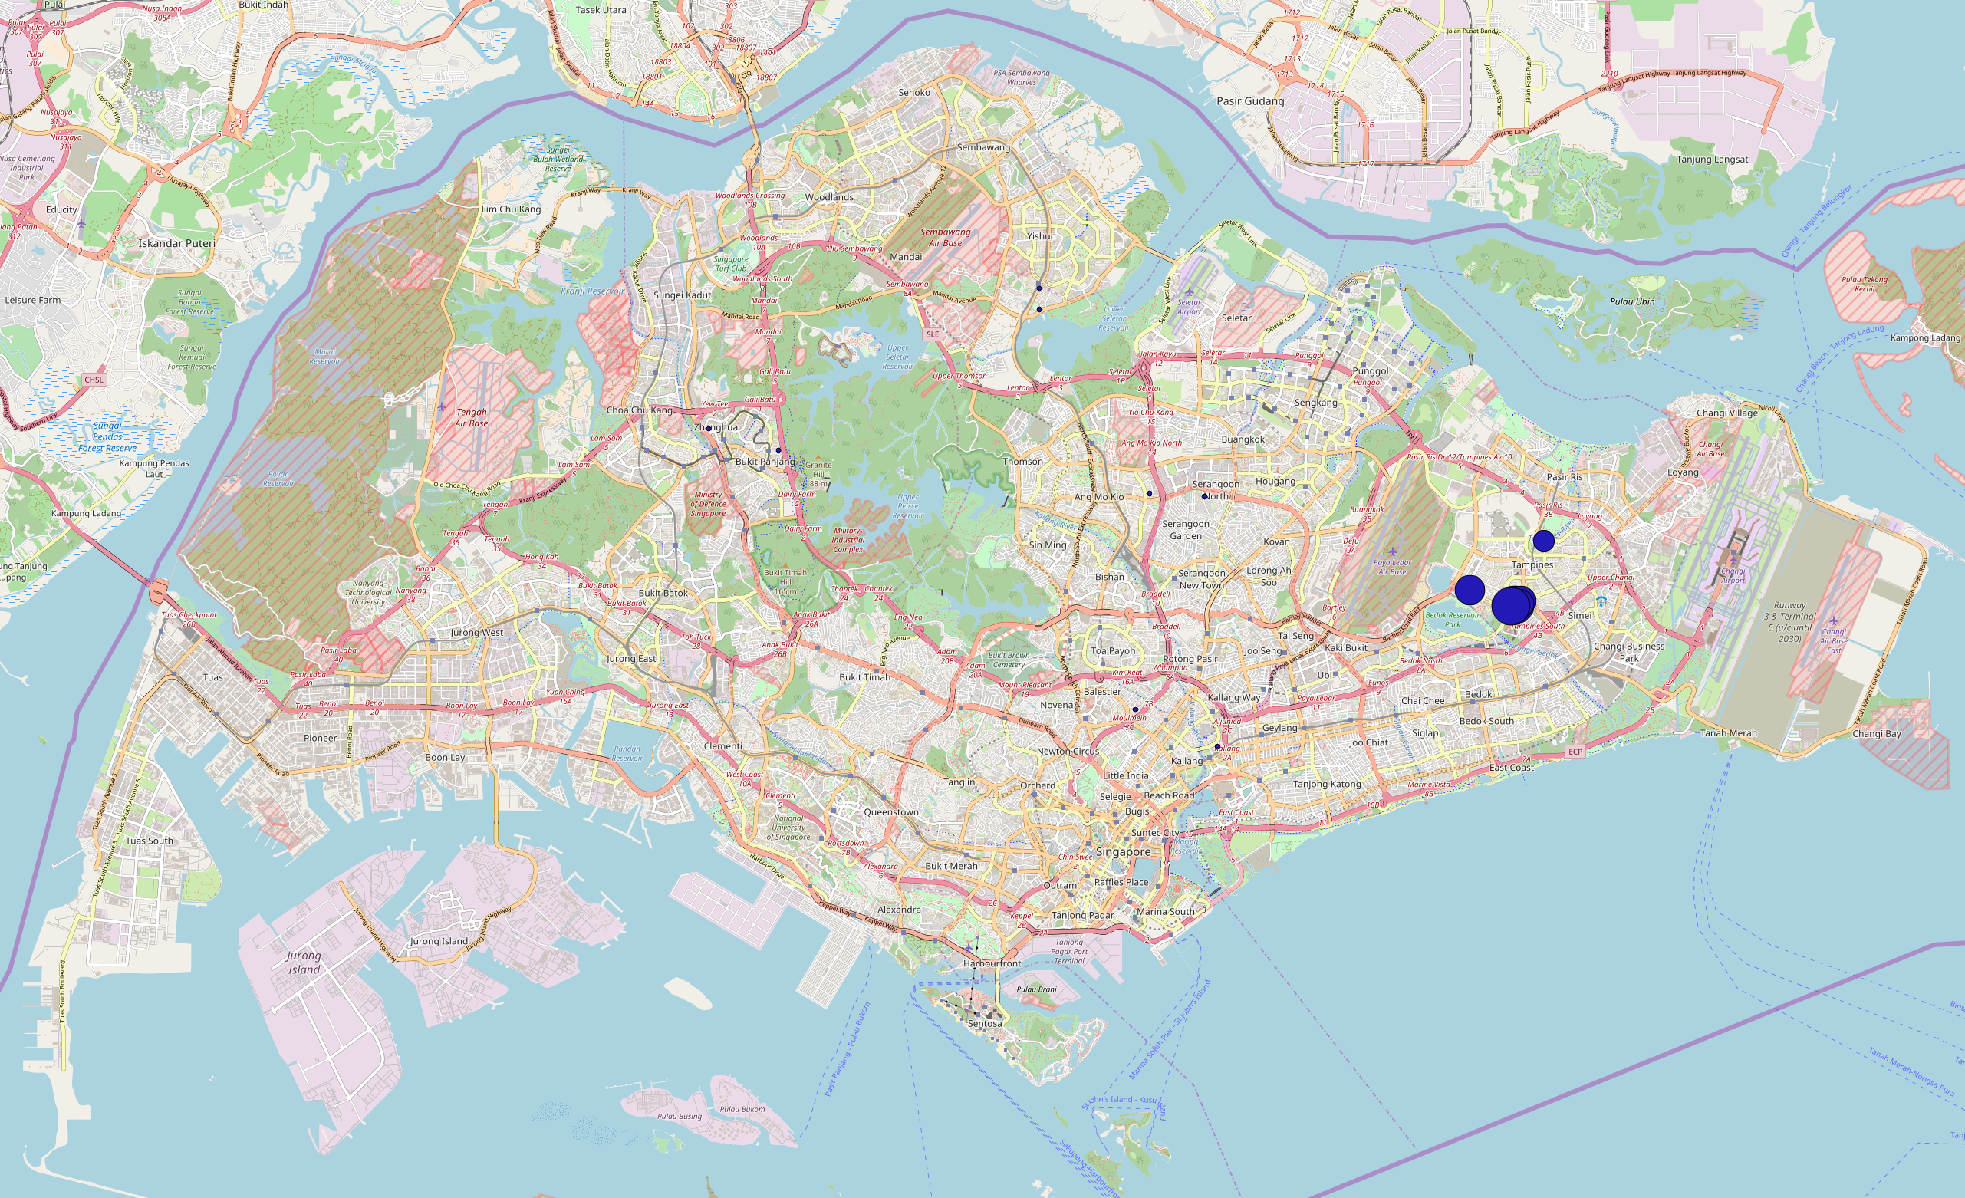
\includegraphics[width=\linewidth]{./assets/201802092147.png}
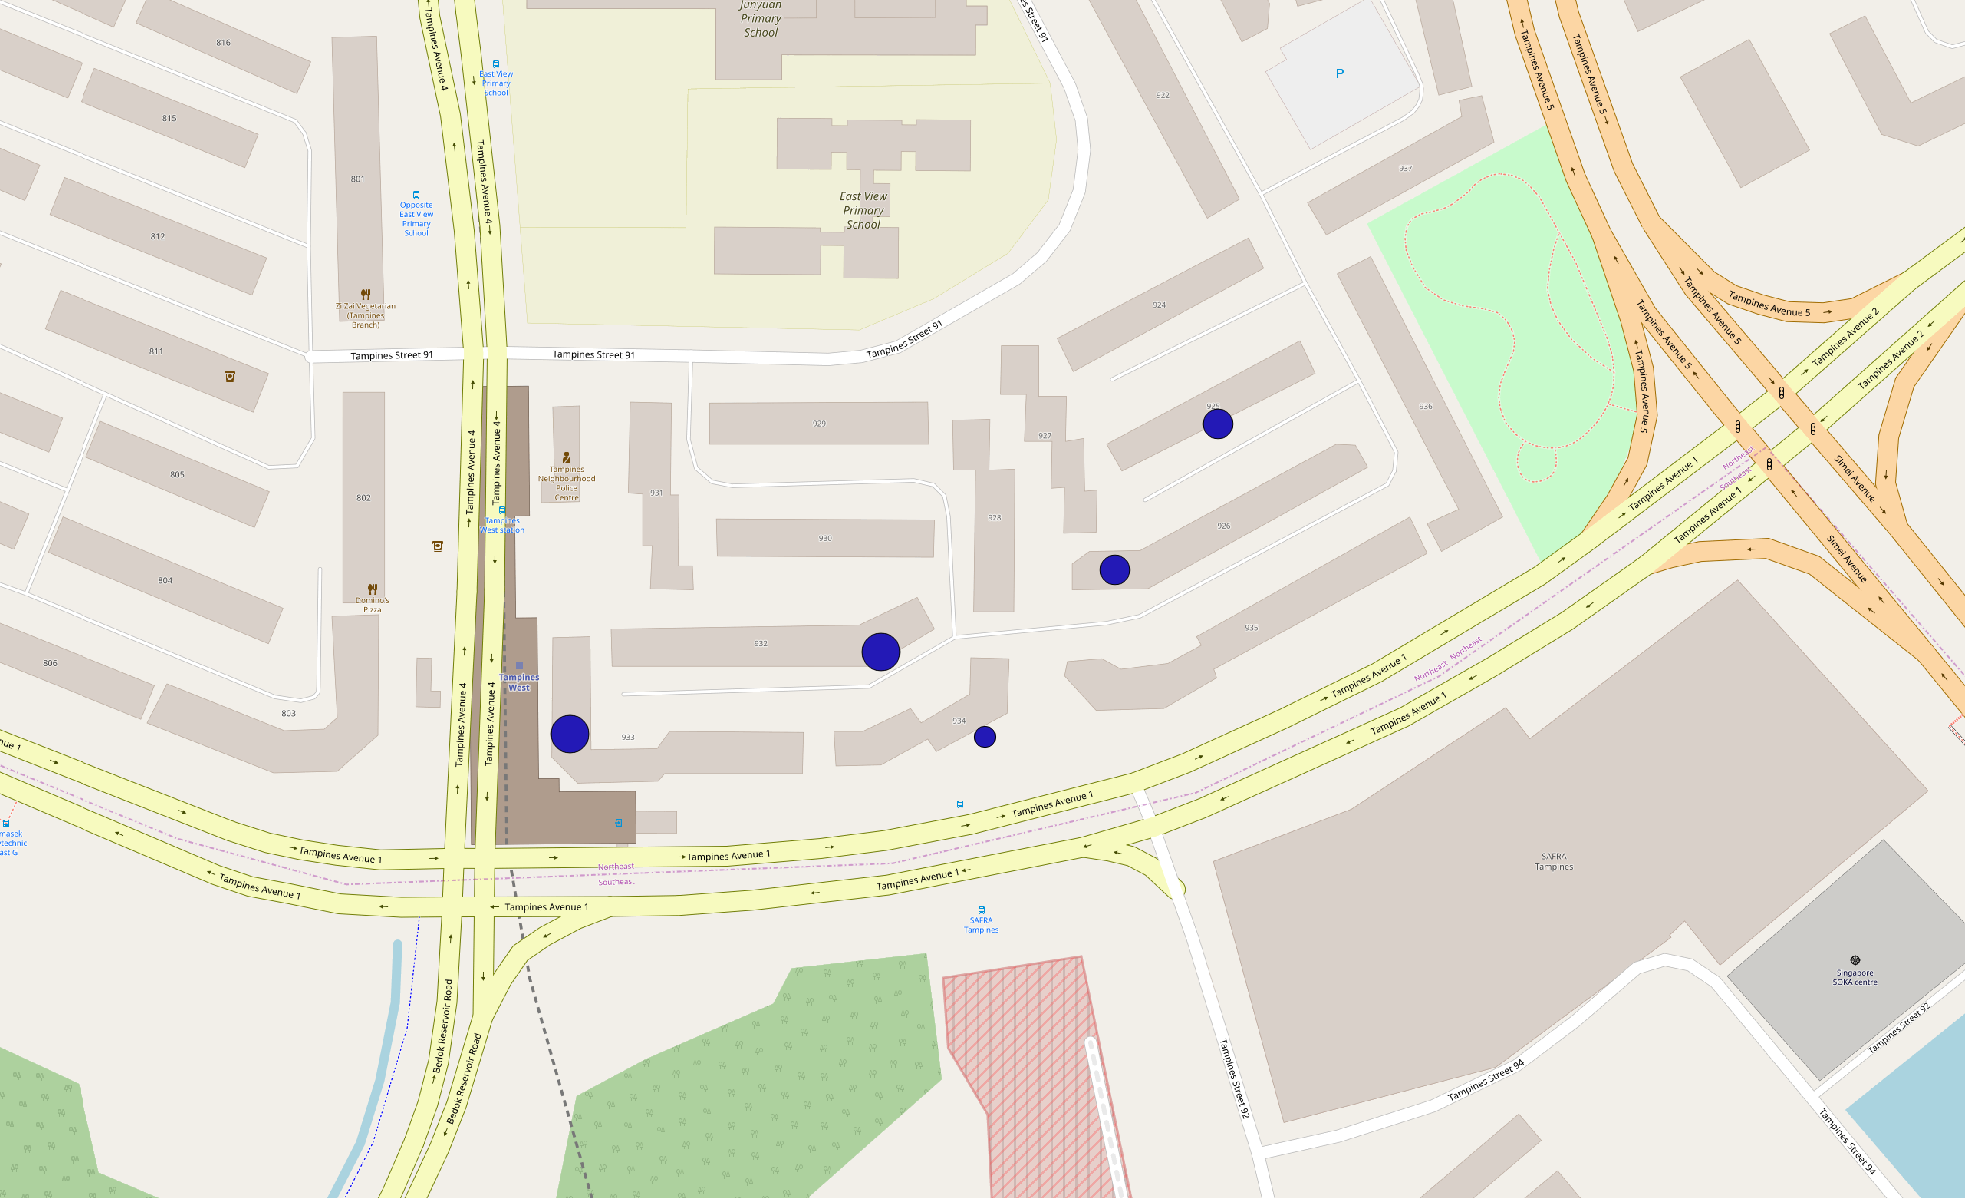
\includegraphics[width=\linewidth]{./assets/201802092151.png}
\caption{Unusual Concentration of Missing Bikes I}
\label{figure:map6}
\end{figure}

\end{itemize}

\end{document}